%\chapter{Vorlesung}
\section{Restnetzwerk $G_f=(V,E_f)$}
\[ c_f(u,v)=\begin{cases}
c(u,v)-f(u,v)&\text{für }(u,v)\in E\\
f(v,u)&\text{für }(v,u)\in E\\
0 & \text{sonst}
\end{cases} \]
\section{Max-Flow-Min-Cut-Theorem}
\begin{enumerate}
	\item $|f|$ ist maximal $\Rightarrow$ Es gibt keinen $f$-verbessernden Pfad
	\item Es gibt einen $(S,T)$-Schnitt, so dass $c(S,T)=|f|$
	\item $c(S,T) = |f| \Rightarrow f$ ist maximal und $c(S,T)$ minimal
\end{enumerate}
\subsection{Beweis: 1. $\Rightarrow$ 2.}
Gegeben sein ein maximaler Fluss $f\Rightarrow  t$ ist in $G_f$ nicht von $s$ erreichbar.
\[ \text{Sei }S=\{ v\in V | \exists~p:~s \rightsquigarrow v \text{ in } G_f \}, T=V\setminus S, t \in T \]
%Wrap left Dia2
\begin{wrapfigure}{L}{0.3\linewidth}
	\centering
	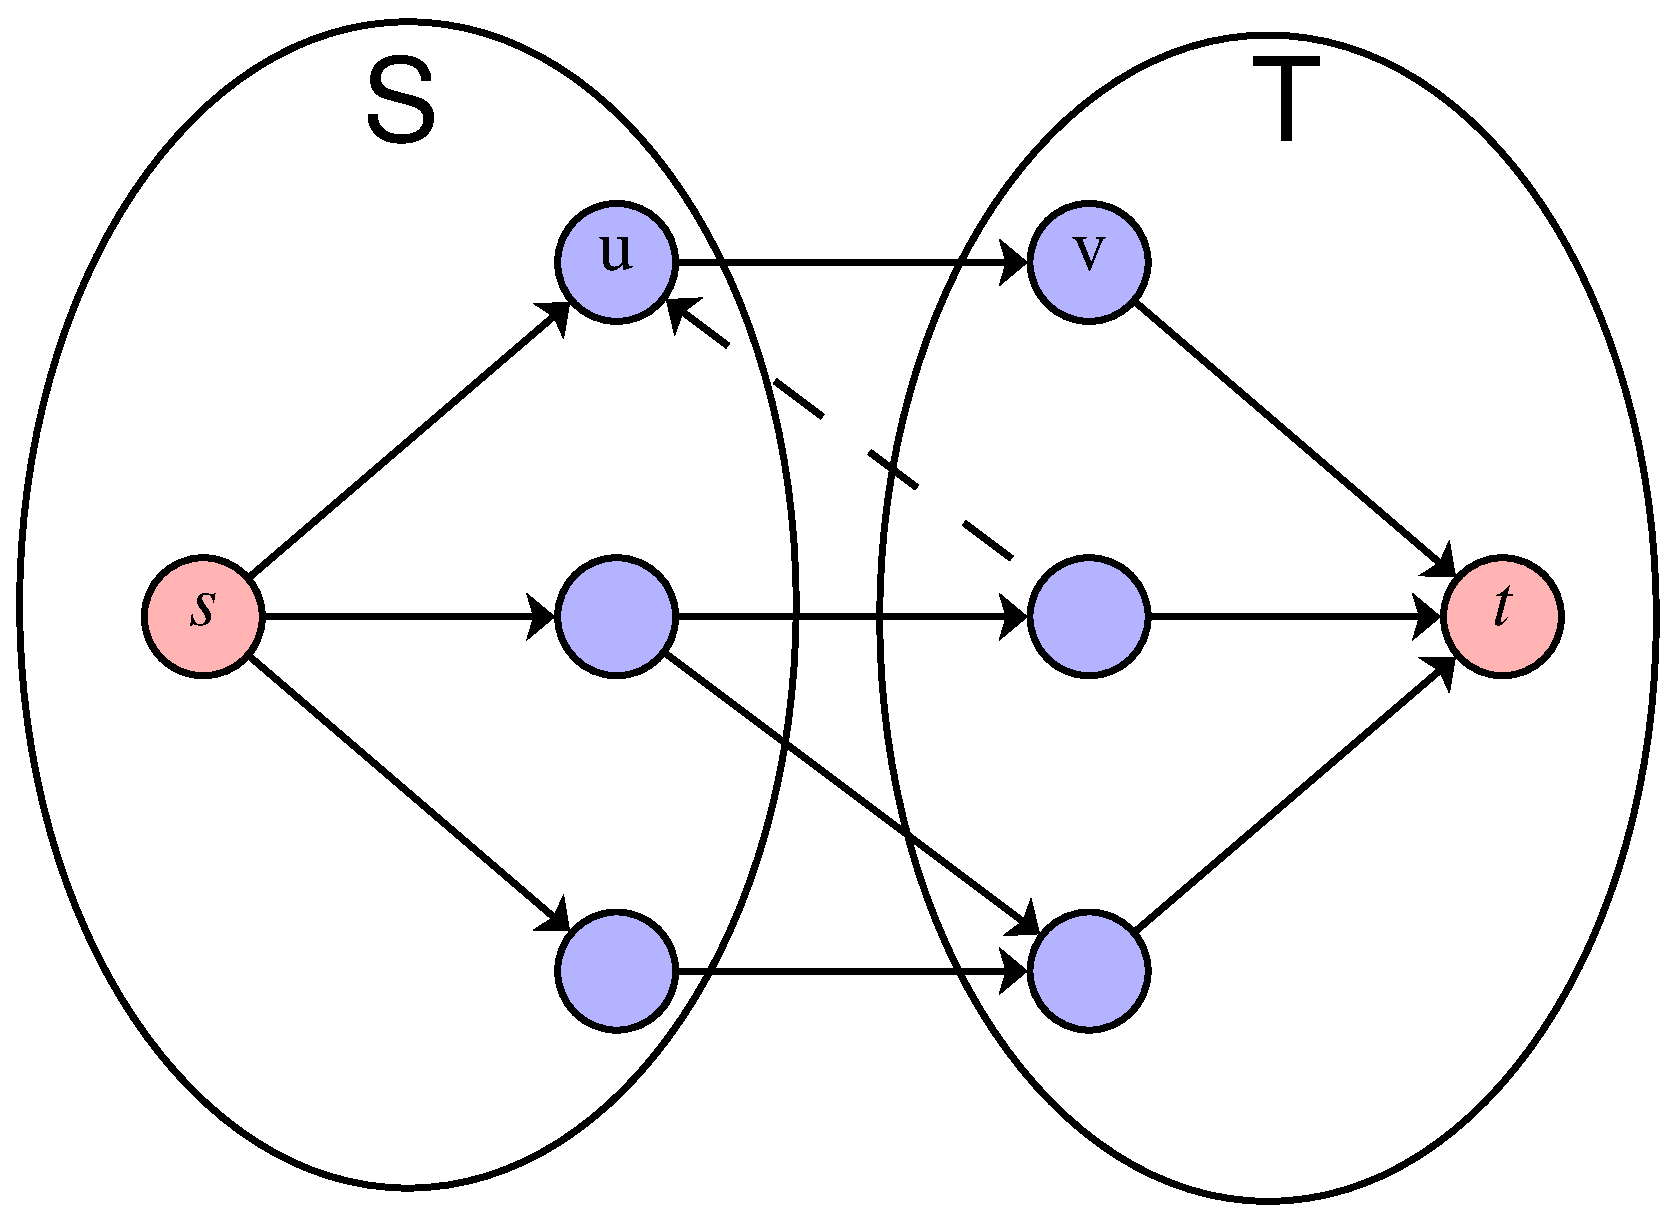
\includegraphics[width=\linewidth]{25/Grafik/Diagramm2}
	\caption{}
\end{wrapfigure}
\subsection{Idee}
\paragraph{Zeige:} Alle Vorwärtskanten über den Schnitt $S,T$ sind saturiert, d.h. $f(u,v)=c(u,v)$ Alle Rückwärtskanten von $T$ nach $S$ tragen den Flusswert $0$.

\paragraph{Beweis}
Sei $(u,v) \in S\times T \cap E$
\subparagraph{Anmerkung} $f(u,v) < c(u,v)$
\[ \Rightarrow (u,v) \in E_f \text{ mit } c_f(u,v)=c(u,v)-f(u,v) > 0 \]
\[ \Rightarrow v \text{ ist von }s\text{ aus erreichbar:} s\rightsquigarrow u \rightarrow v \lightning \] 
\begin{align*}
% \hline
\end{align*}

\pagebreak

Sei $(v,u) \in T\times S$
%Wrap left dia3
\begin{wrapfigure}{L}{0.2\linewidth}
	\centering
	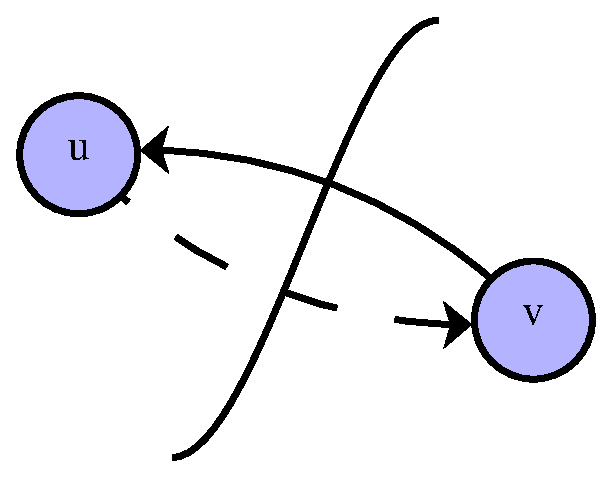
\includegraphics[width=\linewidth]{25/Grafik/Diagramm3}
	\caption{}
\end{wrapfigure}
\subparagraph{Anmerkung:} $f(v,u)>0$
\[ \Rightarrow (u,v)\in E_f\text{ mit } c_f(u,v) = f(v,u)>0 \]
\[ \Rightarrow v \text{ ist auf dem Weg } s\rightsquigarrow u \rightarrow v\text{ in }G_f\text{ erreichbar.}\lightning \]
\[ |f| = \sum_{u\in S, v \in T}f(u,v) - \sum_{u\in S, v\in T}f(v,u) = \sum_{u\in S, v\in T} c(u,v) - 0 = c(S,T) \]
\begin{flushright}
	1. $\Rightarrow$ 2.\\
	q.e.d.
\end{flushright}
\[ |f| = c(S,T) \Rightarrow f\text{ maximal und }c(S,T)\text{ minimal.} \]
\begin{align*}
\hline
\end{align*}
\paragraph{Offene Frage}
Unter welchen Bedingungen terminiert der Ford-Fulkerson-Algorithmus?
\subparagraph{Anmerkung} $c:E\rightarrow \mathbb{N}$ 
\[\Rightarrow |f^*|\footnote{maximaler Fluss}\in \mathbb{N}, c_{min}(p) \in \mathbb{N} \text{ für }p\text{ flussverbessernder Pfad} \geq 1\]
\[ \Rightarrow \text{ Es genügen }|f^*|\text{ viele Iterationen zur Flussverbesserung} \]
\[ \Rightarrow \text{Laufzeit}\mathcal{0}(|f^*|\cdot|E|) \]
%Grafik 4
\begin{figure}[h]
\centering
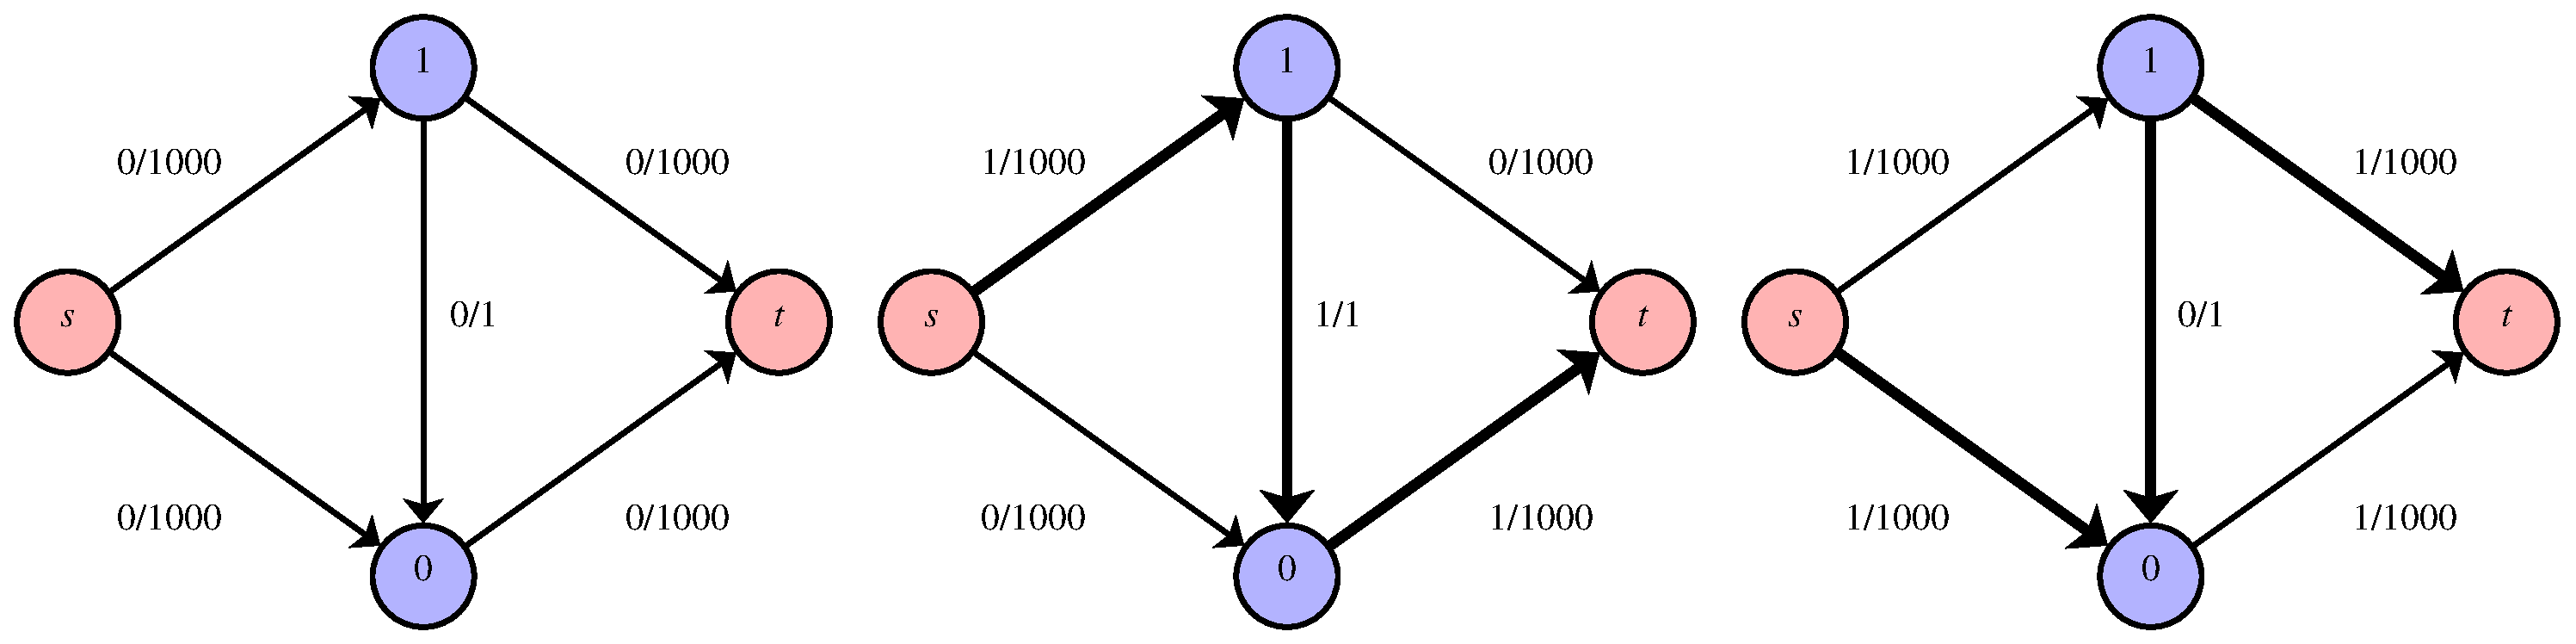
\includegraphics[width=\linewidth]{25/Grafik/Diagramm4}
\caption{}
\label{fig:Diagramm4}
\end{figure}
\pagebreak
\subsection{Zwick}
\[ \overline{\phi} = \frac{\sqrt{5}-1}{2}~~X>1000~~|f^*|=2X+1 \]
\begin{figure}[H]
	\centering
	\begin{subfigure}[H]{0.4\linewidth}
\centering
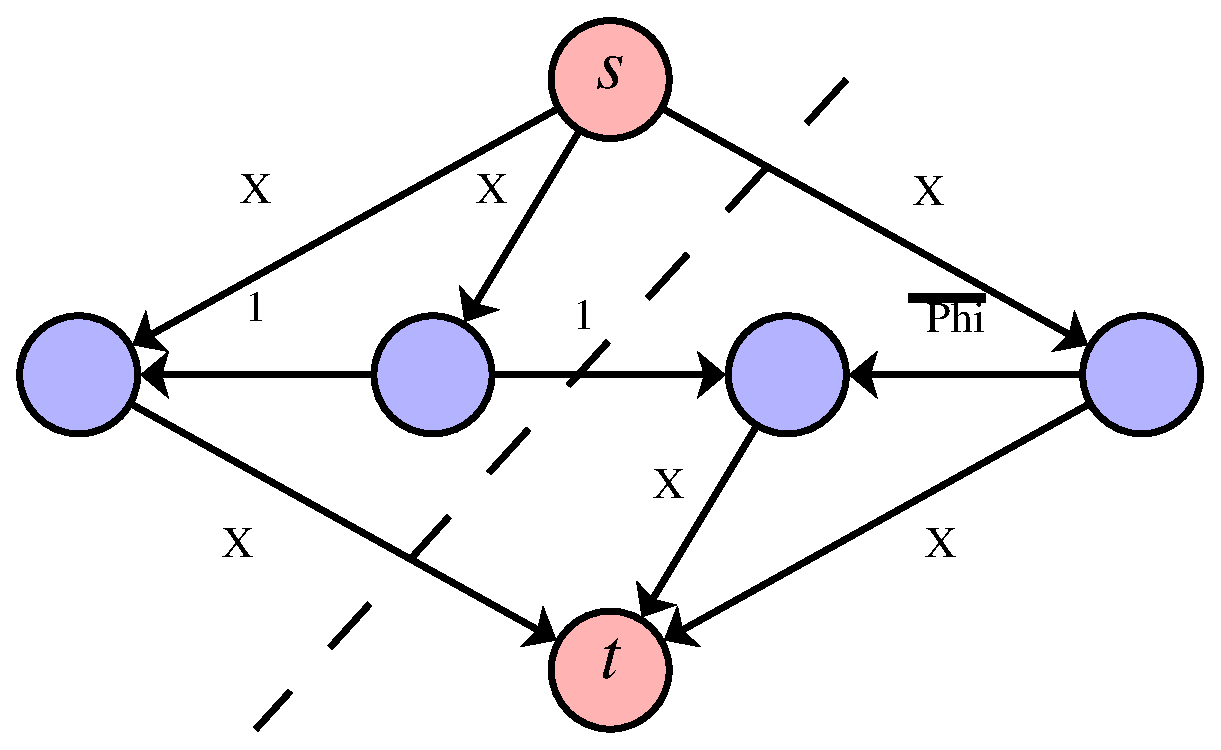
\includegraphics[width=\linewidth]{25/Grafik/Diagramm5}
\caption{}
\label{fig:Diagramm5}
\end{subfigure}
\begin{subfigure}[H]{0.3\linewidth}
\centering
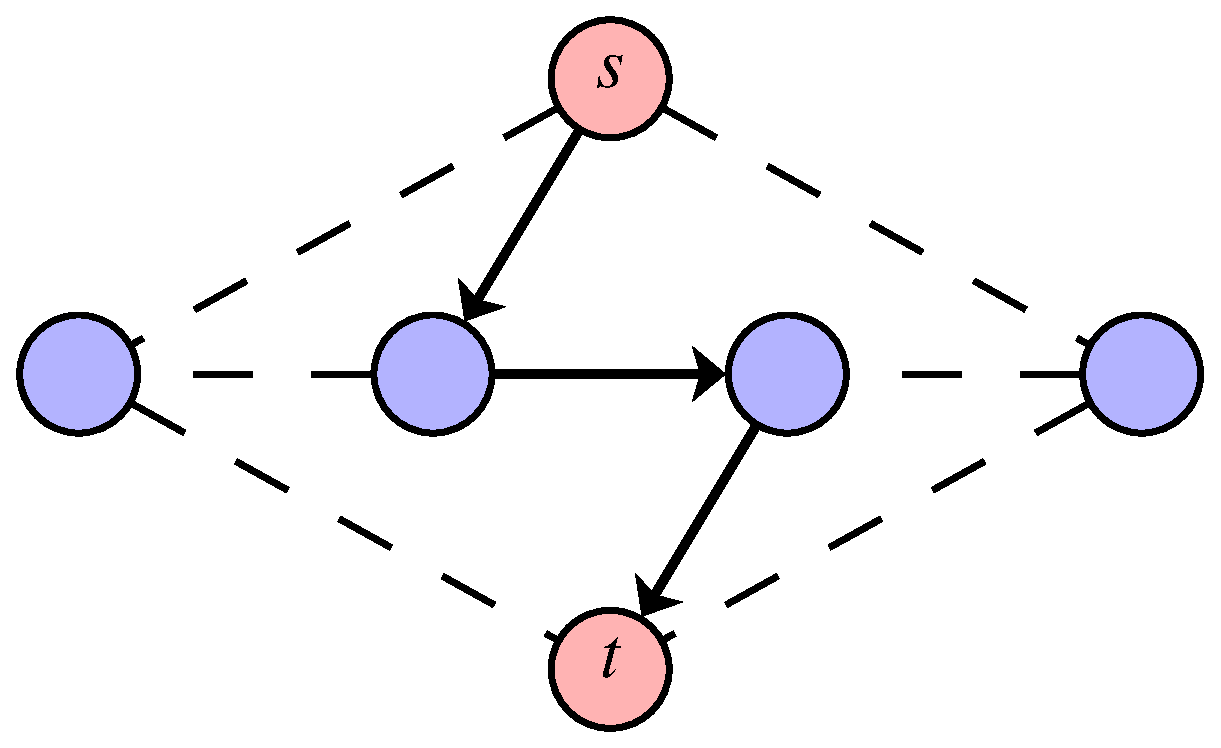
\includegraphics[width=\linewidth]{25/Grafik/ersterSchritt}
\caption{Erster Schritt}
\label{fig:ersterSchritt}
\end{subfigure}
\end{figure}
\begin{figure}[H]
	\centering
	\begin{subfigure}[H]{0.3\linewidth}
		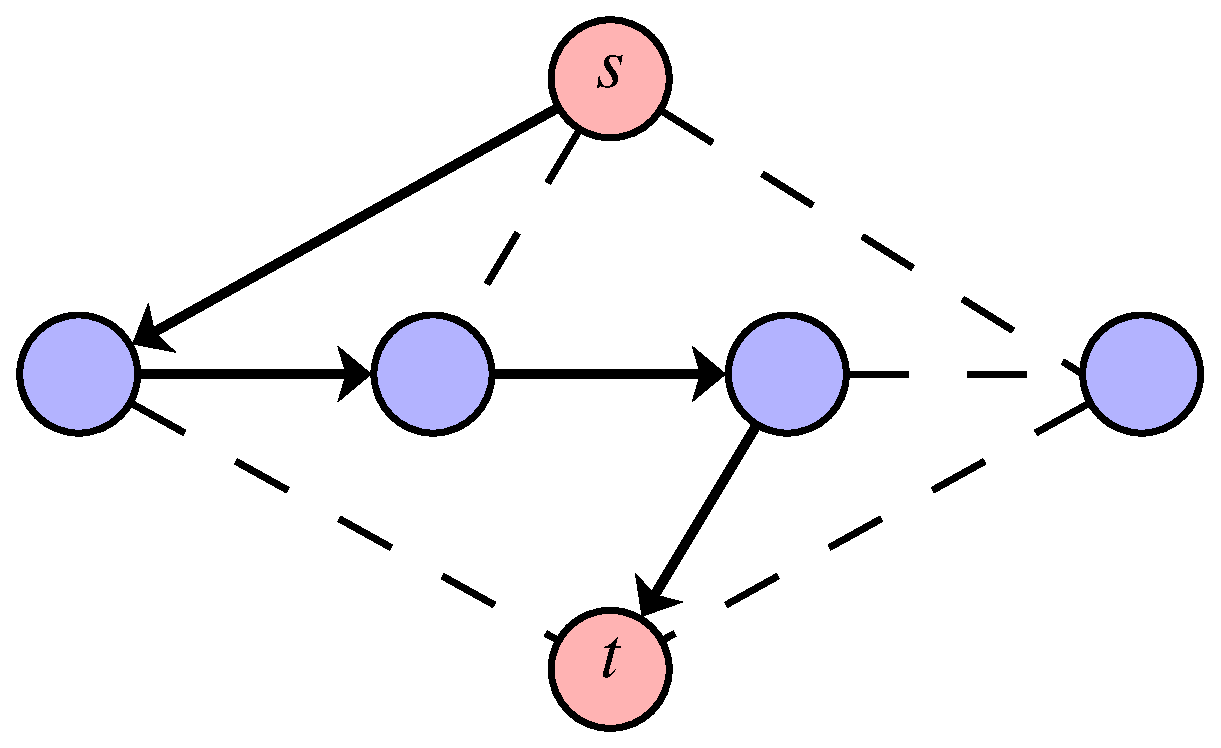
\includegraphics[width=\linewidth]{25/Grafik/PfadA}
		\caption{Pfad A}
	\end{subfigure}
	\begin{subfigure}[H]{0.3\linewidth}
		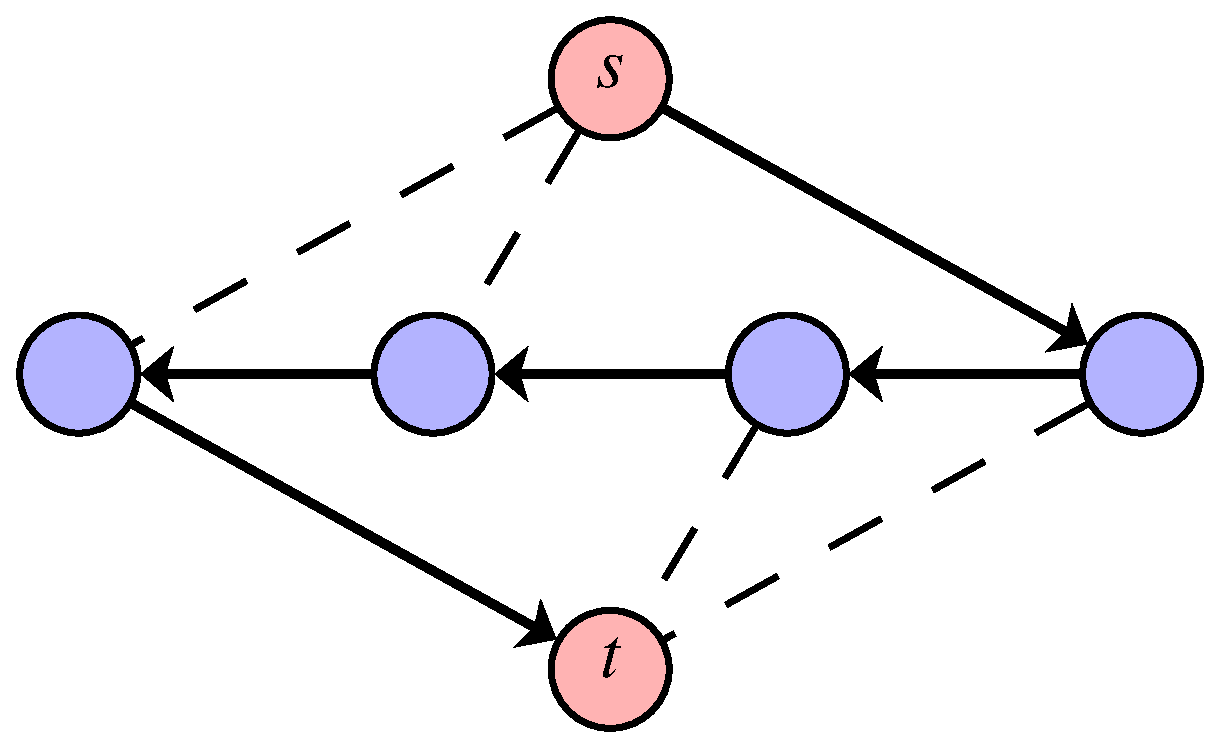
\includegraphics[width=\linewidth]{25/Grafik/PfadB}
		\caption{Pfad B}
		
	\end{subfigure}
	\begin{subfigure}[H]{0.3\linewidth}
		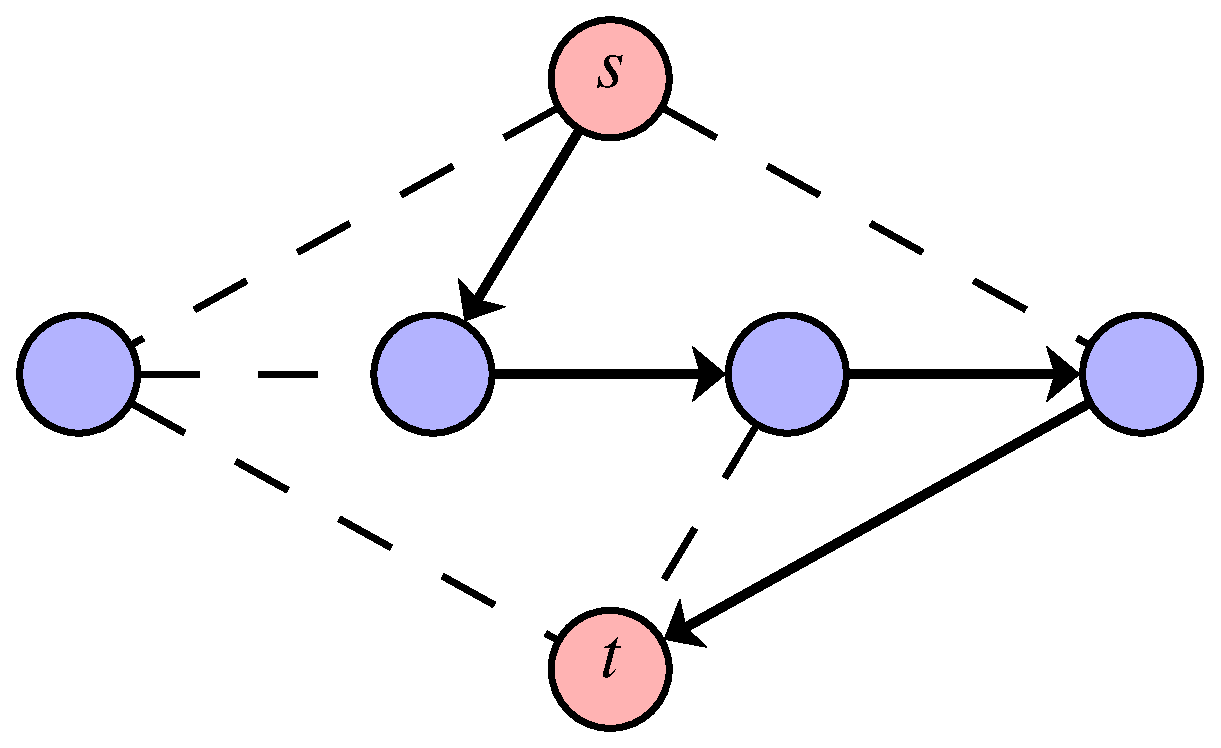
\includegraphics[width=\linewidth]{25/Grafik/PfadC}
		\caption{Pfad C}

	\end{subfigure}
\end{figure}
%Grafik 5
%ersterSchritt und Pfade A-C
\paragraph{Invariante} $\overline{\phi}=0,613\ldots$
\begin{figure}[H]
\centering
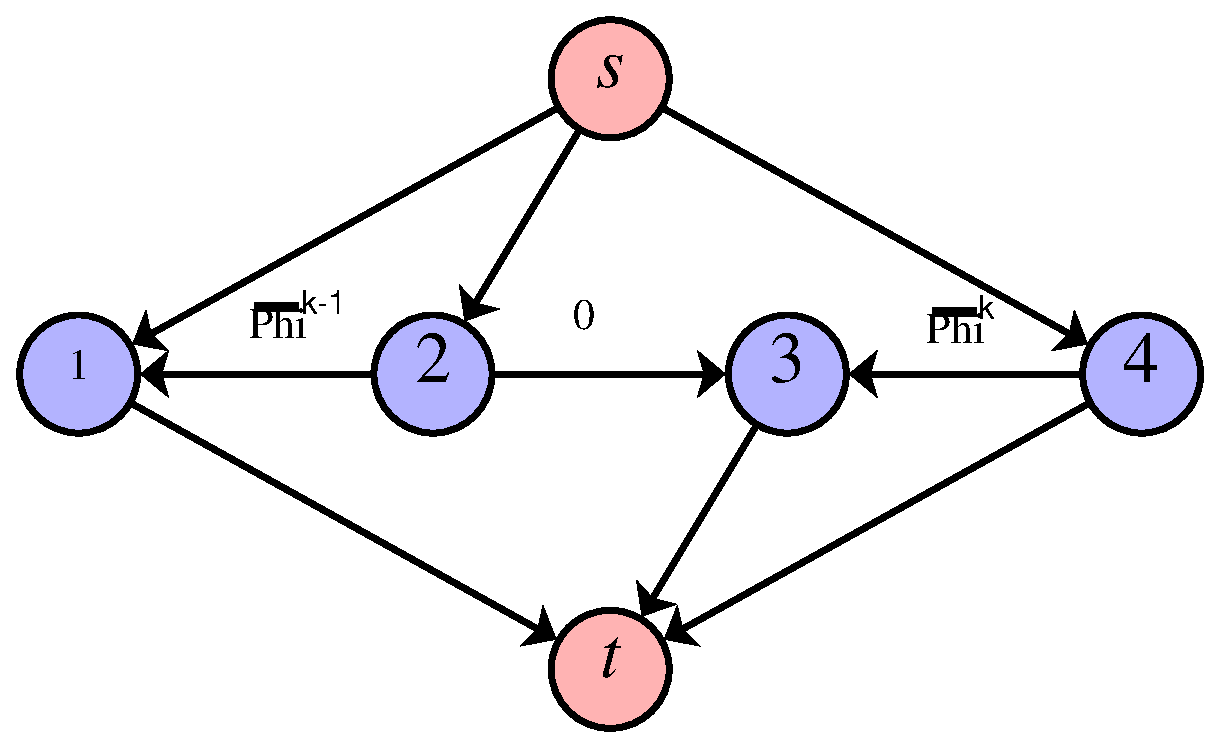
\includegraphics[width=0.4\linewidth]{25/Grafik/Diagramm10}
\caption{}
\label{fig:Diagramm10}
\end{figure}

%Grafik 10
\[1-\overline{\phi}=\overline{\phi}^{~2} \]
\[ \overline{\phi}^{~k-1}-\overline{\phi}^{~k} = \overline{\phi}^{~k+1} \]
\pagebreak
\paragraph{1. Schritt} Schicke $\overline{\phi}^{~k}$ Flusseinheiten entlang Pfad B
\begin{figure}[H]
\centering
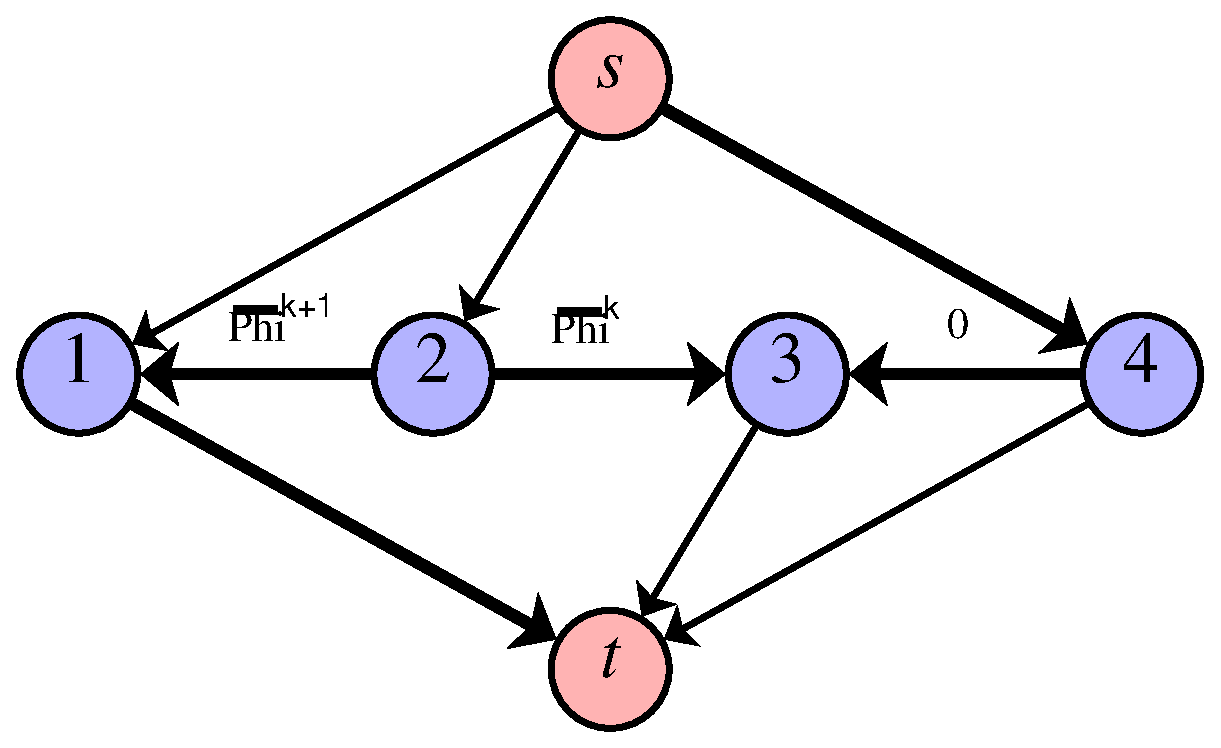
\includegraphics[width=0.3\linewidth]{25/Grafik/Schritt1}
\caption{Schritt 1}
\label{fig:Schritt1}
\end{figure}

%Grafik Schritt1
\paragraph{2. Schritt} Schicke $\overline{\phi}^{~k}$ entlang C
\begin{figure}[H]
\centering
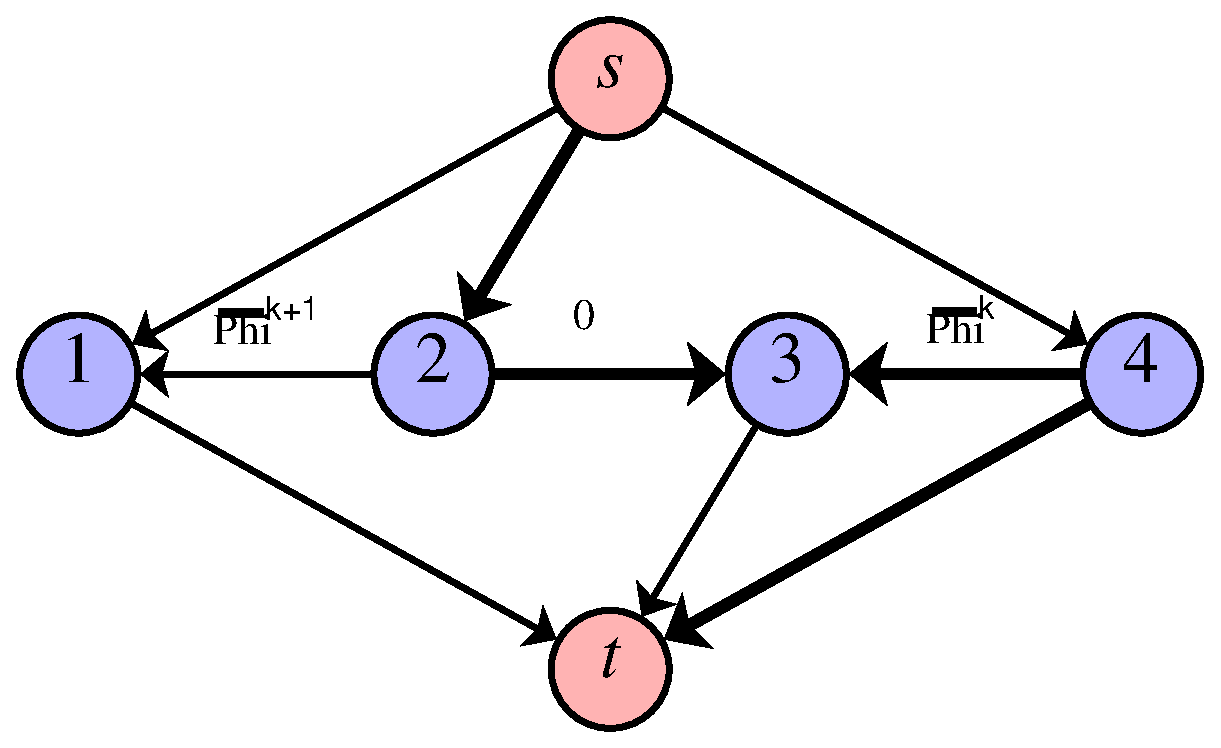
\includegraphics[width=0.3\linewidth]{25/Grafik/Schritt2}
\caption{Schritt 2}
\label{fig:Schritt2}
\end{figure}

%Grafik Schritt2
\paragraph{3. Schritt} Schicke $\overline{\phi}^{~k+1}$ entlang B
\begin{figure}[H]
\centering
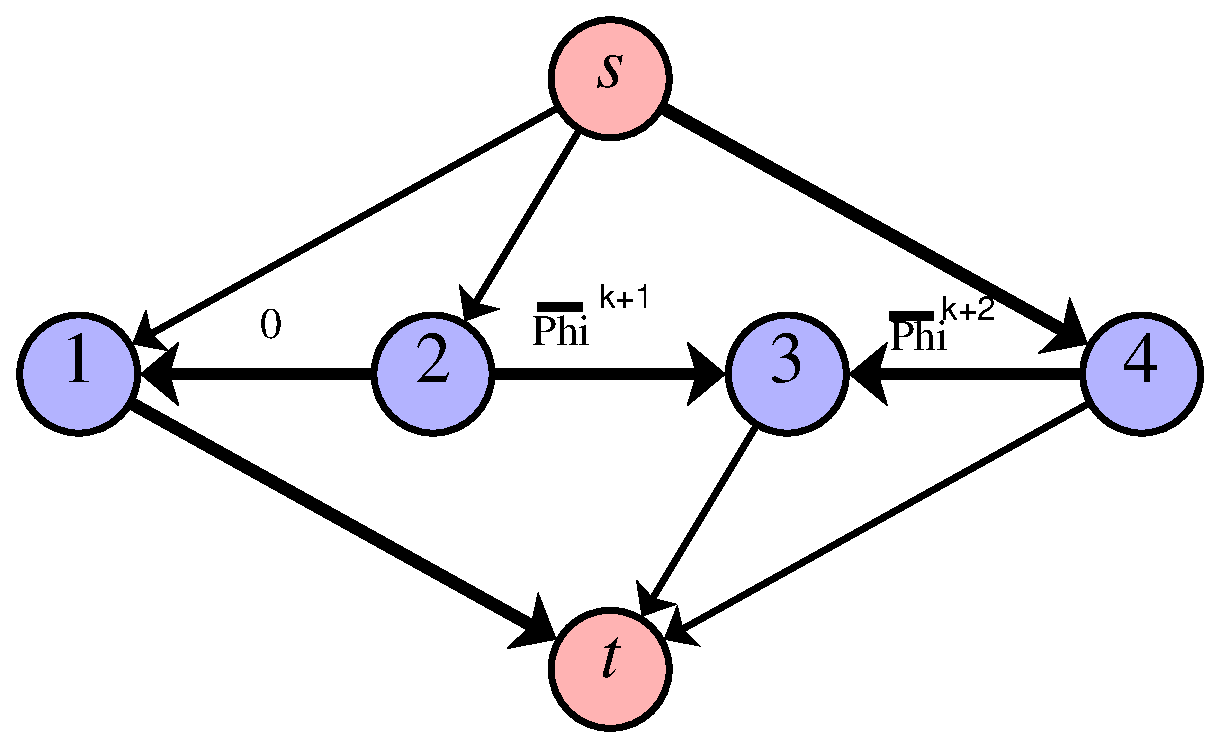
\includegraphics[width=0.3\linewidth]{25/Grafik/Schritt3}
\caption{Schritt 3}
\label{fig:Schritt3}
\end{figure}

%Grafik Schritt3
\paragraph{2. Schritt} Schicke $\overline{\phi}^{~k+1}$ entlang A
\begin{figure}[H]
\centering
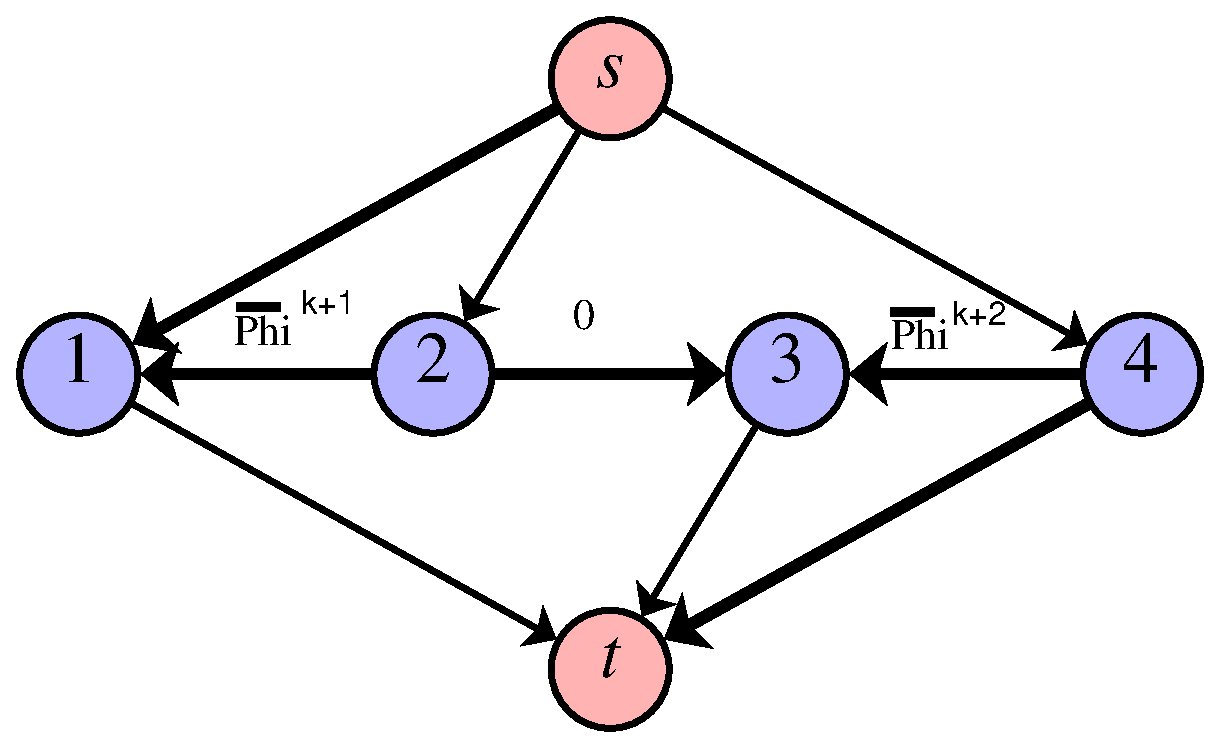
\includegraphics[width=0.3\linewidth]{25/Grafik/Schritt4}
\caption{Schritt 4}
\label{fig:Schritt4}
\end{figure}

%Grafik Schritt4
Wir iterieren diese 4 Schritte unendlich oft
\[ |f| = 1+2\cdot\sum_{k=1}^{\infty}\overline{\phi}^{~k}+2\cdot\sum_{k=1}^{\infty}\overline{\phi}^{~k+1}<7\leq 2X+1~~~~~\sum_{k=0}^{\infty}\overline{\phi}^{~k}=\frac{1}{1-\overline{\phi}} \]